\documentclass[aps,reprint,superscriptaddress,10pt]{revtex4-2}
\usepackage{kotex}
\usepackage[HWP]{dhucs-interword}
\usepackage[dvips]{color}
\usepackage{graphicx}
\usepackage{bm}
\usepackage{amsmath}
\usepackage{tikz}
\usepackage{mhchem}
\usepackage{booktabs}
\usepackage{multirow}
\usepackage{array}
\usepackage{tikz}
\usepackage{tabularx}

\begin{document}
\title{응집물질물리실험 결과보고서 \\
\small 실험주제 : Four point probe resistivity
measurement}

\author{HuiJae-Lee}\email{hjlee6674@inha.edu}
\affiliation{Physics Department, Inha University}

\date{\today}

\begin{abstract}
4  point probe 방법을 통해 Al Foil에서의 비저항이 Si sample의 비저항보다 낮다는
사실과 온도가 높을 때 비저항이 더 높아진다는 사실을 확인할 수 있었다.
  \end{abstract}

 \maketitle
 
 \section{Process}
 \subsubsection{For matter}
 \begin{itemize}
     \item[1. ]
     4 point probe 장비와 Voltage meter, Current source를 연결선을 통해 연결한다.
     \item[2. ]
     4 point probe 장비와 Oven을 연결한다.
     \item[3. ]
     4 point probe의 샘플 스테이지에 시료를 놓는다. 이때, 4 point probe 장비에 
     적절한 압력을 주어 탐침과 시료가 닿도록 만들고, 나사를 조여 고정한다. 
     \item[4. ]
     Oven의 스위치를 set으로 올려주고 다이얼을 돌려 25℃로 설정해준다.
     \item[5. ]
     Current source와 Voltage meter의 스케일을 적절히 설정하고, 영점을 맞춘다.
     \item[6. ]
     Current source의 다이얼을 돌려 4 point probe의 전류를 증가시키며, 
     이에 따른 전압을 Voltage meter로 측정한다.
     \item[7. ] 
     측정한 전압과 전류 사이의 관계식을 사용하여 시료의 종류에 
     따른 비저항과 면저항을 계산한다. 
     \begin{align}
         \rho = \frac{\pi TV}{\ln{2I}}\approx 4.532\frac{TV}{I},\,\,\,
         \rho_s = \frac{\rho}{T}\approx 4.532\frac{V}{I}
     \end{align}
 
 \end{itemize}
 
 
 \subsubsection{For temperature}
 \begin{itemize}
     \item[1. ]
     Oven의 스위치를 set으로 올려주고 다이얼을 돌려 원하는 값을 설정해준다.
     \item[2. ]
     설정한 값이 일정하게 유지되고 있는 지를 Display를 통해 확인한다. 
     \item[3. ]
     Current source의 다이얼을 조금씩 돌려가며 전류가 증가함에 따라 변화하는 전압을 
     Voltage meter로 측정한다. 
     \item[4. ]
     Oven의 다이얼을 돌려 기존의 값과 다른 온도를 설정해준다.
     \item[5. ]
     2, 3번 과정을 반복한다. 
     \item[6. ]
     전류와 전압 사이의 관계를 이용하여 온도에 따른 비저항을 구하고, 
     온도와 비저항이 어떤 관계를 가지는 지 분석한다.
 
 \end{itemize}

\section{Result}
\subsection{Al Foil, 0.018 mm, 25 C$^\circ$}
\begin{figure}[htbp]
    \centering
    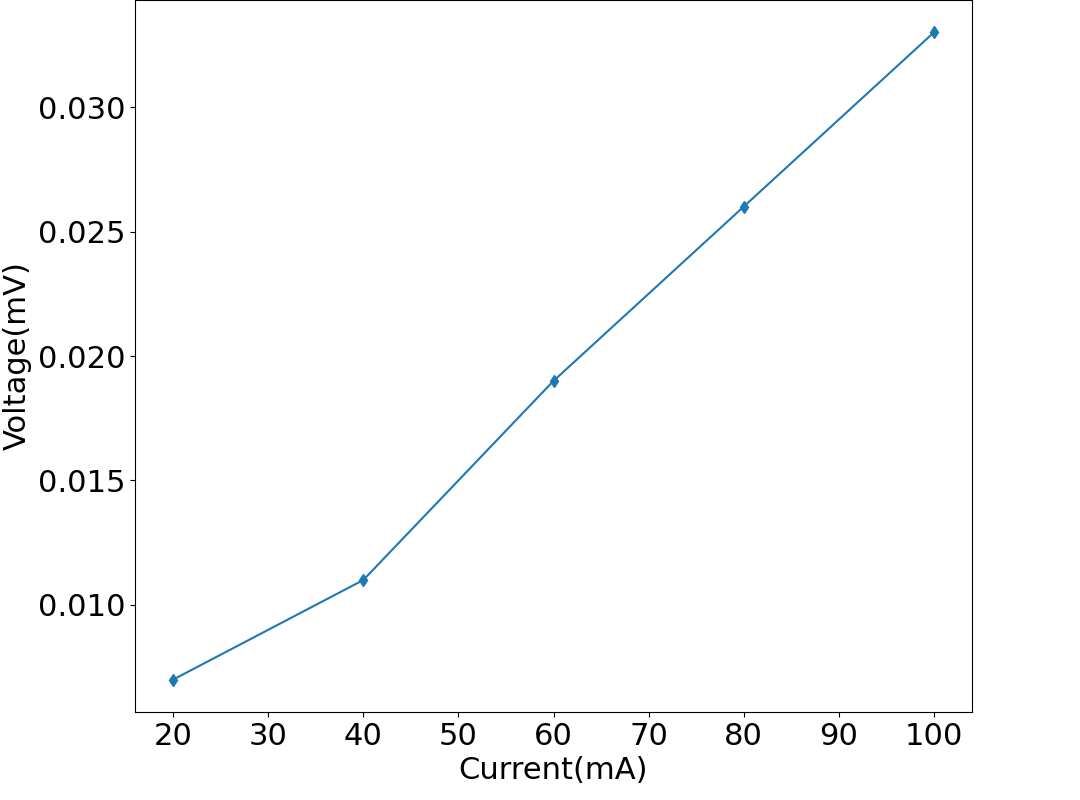
\includegraphics[scale = 0.25]{Al1.png}
    \caption{25 C$^\circ$ 조건에서 4 point probe 장비로 측정한 
    두께 0.018 mm Al Foil의 전류, 전압 관계}
    \label{Al1}
  \end{figure}

  \begin{table}[htp]
    \centering
    \begin{tabular}{>{\centering}p{0.12\textwidth}
      >{\centering}p{0.12\textwidth}
      >{\centering\arraybackslash}p{0.12\textwidth}}
        \toprule
        Current (mA)& $\rho$ ($\Omega\cdot$m) & $\rho_s$ ($\Omega$) \\
        \midrule
        20 &2.9 $\times 10^{-8}$& 1.6 $\times 10^{-3}$\\
        40 &2.2 $\times 10^{-8}$& 1.2 $\times 10^{-3}$ \\
        60 &2.6 $\times 10^{-8}$& 1.4 $\times 10^{-3}$\\
        80 &2.7 $\times 10^{-8}$& 1.5 $\times 10^{-3}$\\
        100&2.7 $\times 10^{-8}$& 1.5 $\times 10^{-3}$\\
        \bottomrule
    \end{tabular}
    \caption{25 C$^\circ$ 조건에서 두께 0.018 mm Al Foil의
    비저항과 면저항}\label{table:1}
  \end{table}
  


\subsection{Al Foil, 0.018 mm, 100 C$^\circ$}
\begin{figure}[htbp]
    \centering
    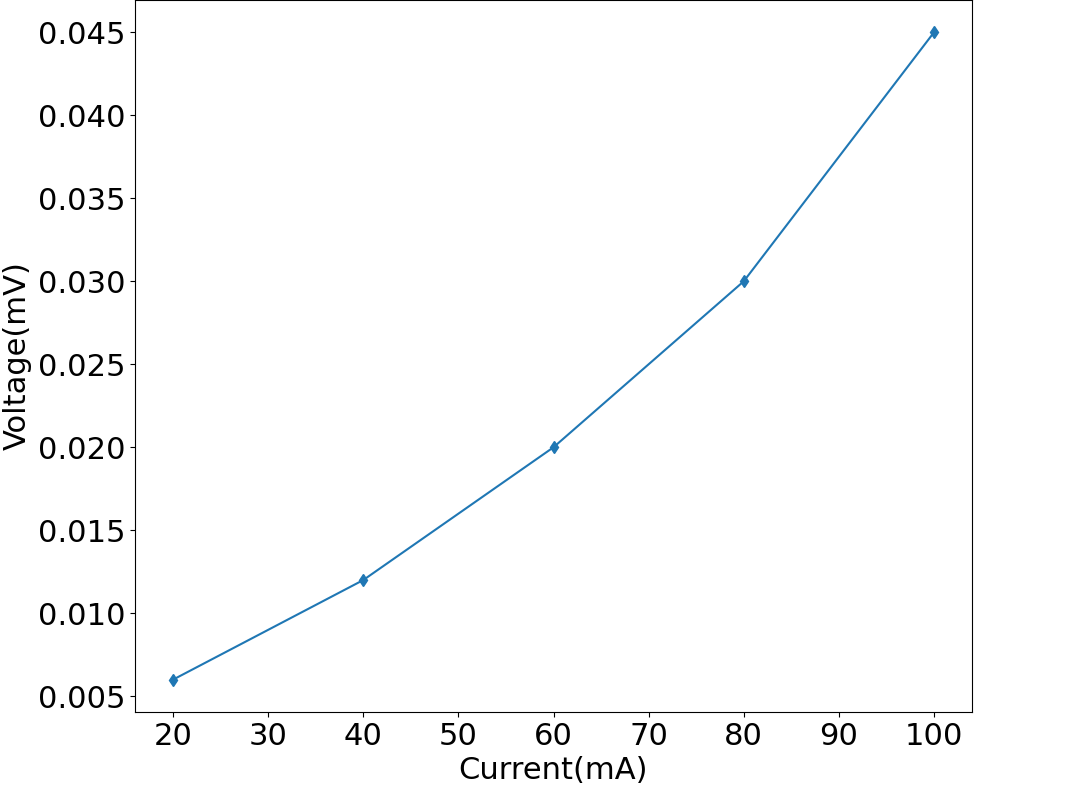
\includegraphics[scale = 0.25]{Al2.png}
    \caption{100 C$^\circ$ 조건에서 4 point probe 장비로 측정한 
    두께 0.018 mm Al Foil의 전류, 전압 관계}
    \label{Al2}
  \end{figure}

  \begin{table}[htp]
    \centering
    \begin{tabular}{>{\centering}p{0.12\textwidth}
      >{\centering}p{0.12\textwidth}
      >{\centering\arraybackslash}p{0.12\textwidth}}
        \toprule
        Current (mA)& $\rho$ ($\Omega\cdot$m) & $\rho_s$ ($\Omega$) \\
        \midrule
        20 &2.4 $\times 10^{-8}$& 1.4 $\times 10^{-3}$\\
        40 &2.4 $\times 10^{-8}$& 1.4 $\times 10^{-3}$ \\
        60 &2.7 $\times 10^{-8}$& 1.5 $\times 10^{-3}$\\
        80 &3.1 $\times 10^{-8}$& 1.7 $\times 10^{-3}$\\
        100&3.7 $\times 10^{-8}$& 2.0 $\times 10^{-3}$\\
        \bottomrule
    \end{tabular}
    \caption{100 C$^\circ$ 조건에서 두께 0.018 mm Al Foil의
    비저항과 면저항}\label{table:2}
  \end{table}



\subsection{Si, 0.50mm, 25 C$^\circ$}
\begin{figure}[htbp]
    \centering
    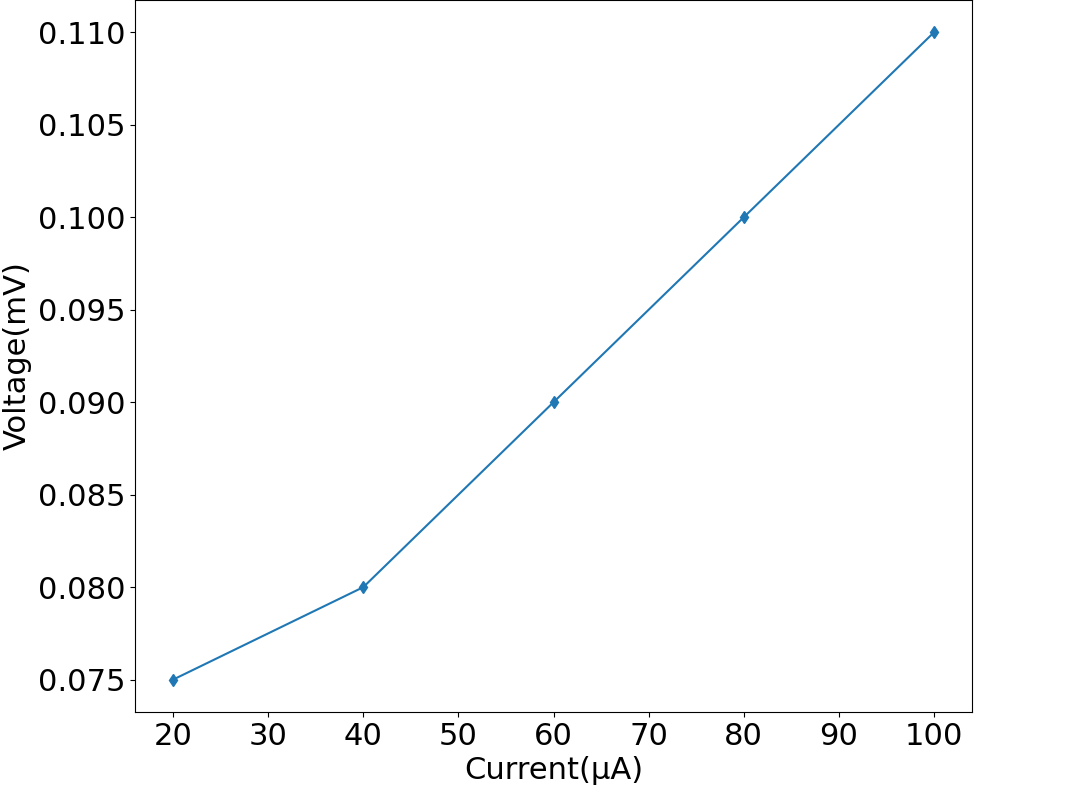
\includegraphics[scale = 0.25]{Si.png}
    \caption{Si, n, 1~10$\Omega$ cm, 0.50mm, 25 C$^\circ$ 조건에서 
    4 point probe 장비로 측정한 두께 0.50 mm
    n형 Si sample의 전류, 전압 관계}
    \label{Si}
  \end{figure}

  \begin{table}[htp]
    \centering
    \begin{tabular}{>{\centering}p{0.12\textwidth}
      >{\centering}p{0.12\textwidth}
      >{\centering\arraybackslash}p{0.12\textwidth}}
        \toprule
        Current (mA)& $\rho$ ($\Omega\cdot$m) & $\rho_s$ ($\Omega$) \\
        \midrule
        20 &8.5 $\times 10^{-3}$& 17  \\
        40 &4.5 $\times 10^{-3}$& 9.1  \\
        60 &3.4 $\times 10^{-3}$& 6.8 \\
        80 &2.8 $\times 10^{-3}$& 5.7 \\
        100&2.5 $\times 10^{-3}$& 5.0 \\
        \bottomrule
    \end{tabular}
    \caption{25 C$^\circ$ 조건에서 두께 0.50 mm Si sample의
    비저항과 면저항}\label{table:3}
  \end{table}

\section{Analysis}
\subsubsection{For matter}
Al Foil과 Si sample에 대해 4 point probe 방법으로 전류에 따른 전압을
측정한 결과, Si sample의 전압이 더 높게 관찰되었고 비저항과 면저항을 비교해보면 
Si sample의 비저항과 면저항이 더 높았음을 확인할 수 있었다. 그래프 FIG.~\ref{AlSi}에서
Si sample은 $\mu$A 스케일에서 측정이 이루어졌다. 이는 Al와 Si가 각각 도체와 반도체의
성질을 가지고 있기 때문으로 해석할 수 있다.


\begin{figure}[htbp]
  \vspace{0.5cm}
  \centering
  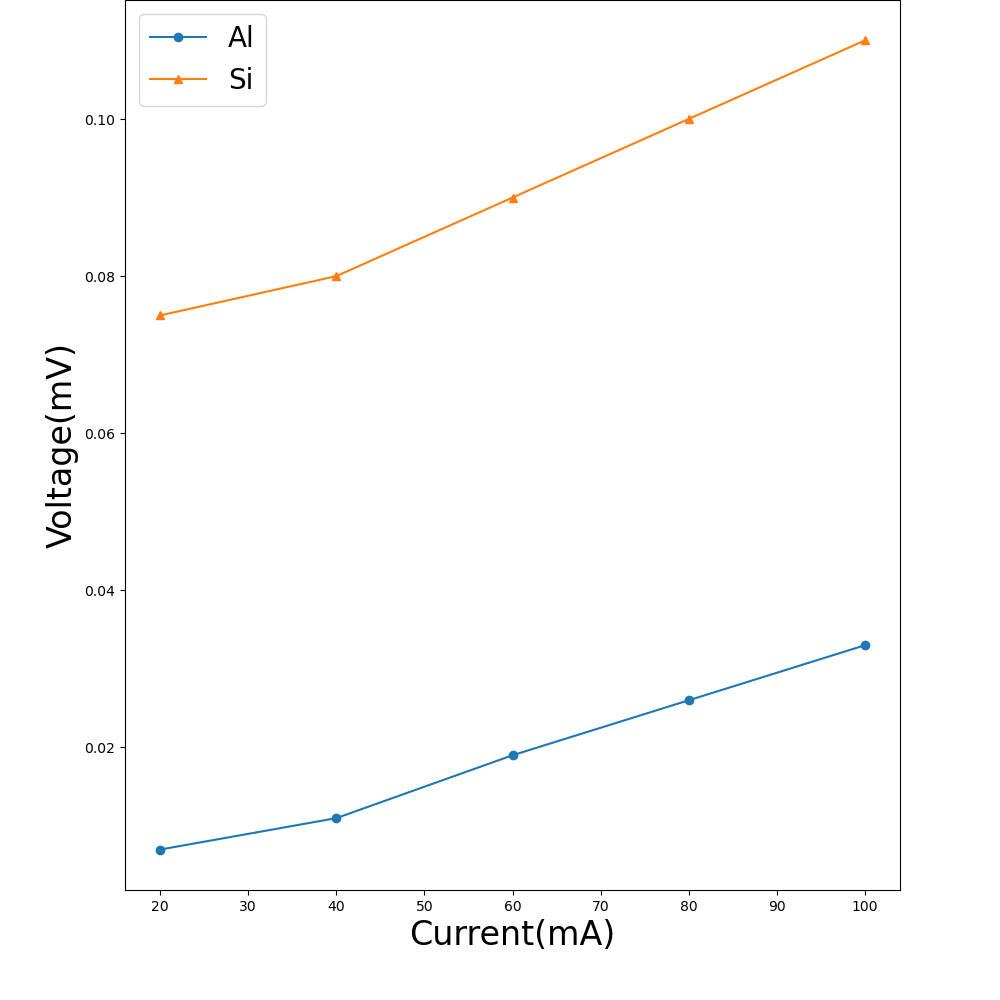
\includegraphics[scale = 0.25]{AlSi.png}
  \caption{두께 0.018 mm Al Foil와 두께 0.50 mm
  n형 Si sample을 각각 25 C$^\circ$ 조건에서
  측정한 그래프}
  \label{AlSi}
\end{figure}



\subsubsection{For temperature}
같은 Al Foil의 온도를 달리하여 4 point probe 방법으로 전류에 따른 전압을
측정한 결과, 온도가 높은 경우에 전압이 더 크게 측정되었고 계산한 비저항과 
면저항 또한 높게 확인되었다. 이는 온도가 높아지면서 분자들의 진동운동이 커지고
전자의 흐름에 더 많은 영향을 주기 때문이다.

  \begin{figure}[htbp]
    \vspace{0.5cm}
    \centering
    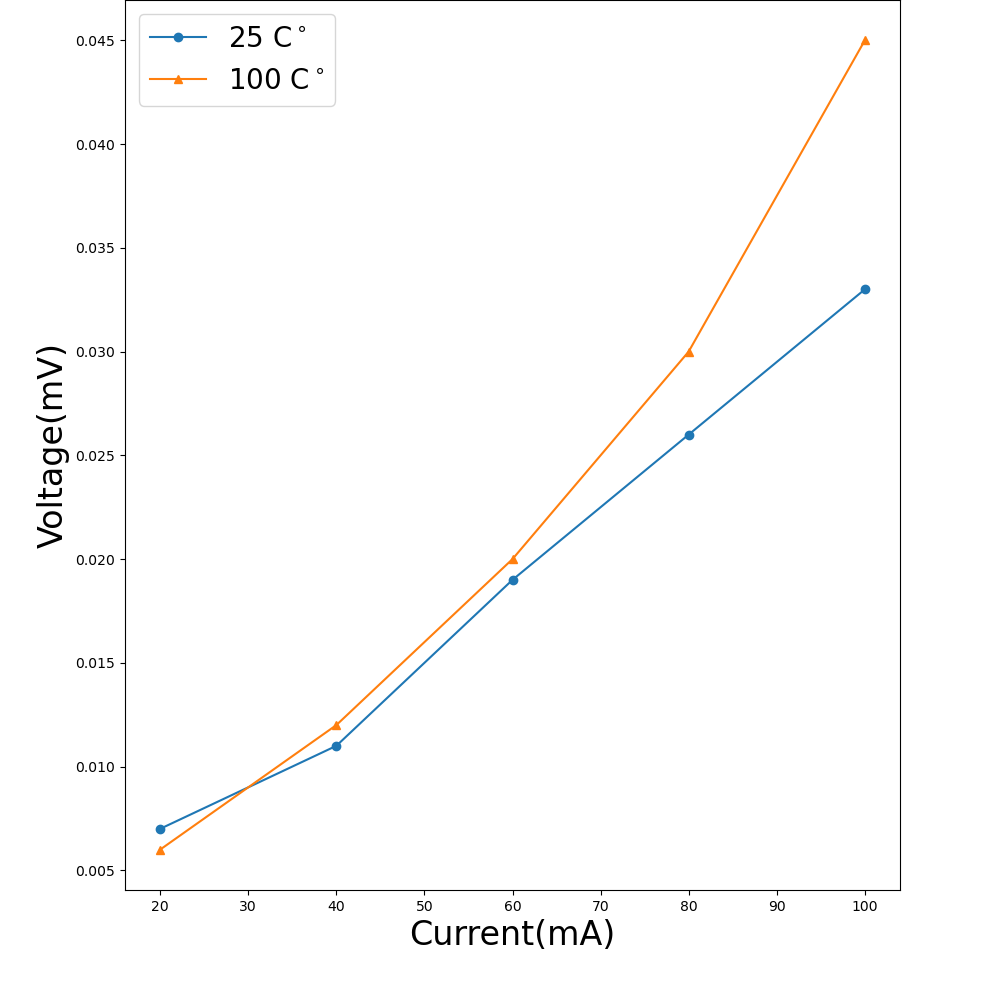
\includegraphics[scale = 0.25]{AlAl2.png}
    \caption{두께 0.018 mm Al Foil을 25 C$^\circ$, 100 C$^\circ$ 조건에서
    각각 측정한 그래프}
    \label{AlAl2}
  \end{figure}



\section{Conclusion}
\begin{itemize}
  \item[1. ]
  Al Foil과 Si sample의 비교를 통해 도체가 반도체보다 4 point probe 방법에 의한
  비저항, 면저항 측정치가 더 낮음을 확인할 수 있었다.
  \item[2. ]
  같은 Al Foil의 온도를 달리하여 측정한 실험의 비교를 통해 온도가 높을 때
  비저항, 면저항 측정치가 더 높음을 확인할 수 있었다.
\end{itemize}


% \nocite{*} 
% \bibliography{ref}



%\begin{thebibliography}{9}
%\end{thebibliography}

\vfill
\end{document}